\documentclass[11pt]{article}
\usepackage[margin=0.85in]{geometry}
\usepackage{amsmath,amssymb,graphicx,hyperref}
\setlength{\parindent}{0pt}\setlength{\parskip}{7pt}
\setlength{\emergencystretch}{3em}
\begin{document}
{\Large Quotient moments: three-support control verified}\\
November 13, 2026. Unsigned producer evidence [pcc:unverified].

\textbf{Role.} This checks the earlier explicit prediction using a supplied,
known norm witness $A,B$. It tests certificate construction and recovery,
not finding that witness from public data.

\textbf{General pairing foundation.} For any field, monic $F$, and nonzero
$P$ with $\deg P<\deg F$, Lean constructs a polynomial $Q$ below $F$ with
\[
 [X^{\deg F-1}]((PQ)\bmod F)\ne0.
\]
A complementary monomial suffices. If $\gcd(F,U)=1$, the same detection is
possible for $PUQ\bmod F$. No characteristic or separability assumption is
needed. These are polynomial detection lemmas; the complete general
Hankel-radical theorem remains a separate obligation.

\textbf{Exact control.} Over $\mathbb F_{17}$ take
\[
 f=X^3+2X+2,\quad A=5X^2+11X+6,\quad B=1,\qquad
 A^2-fB^2=8X(X-5)(X-6)(X-3).
\]
For $\widehat A=(X-16)(X-9)$ and $U=7X+6$, the inverse identity is checked.
For every polynomial $P$ over $\mathbb F_{17}$,
\[
 \mu(P)=[X]((PU)\bmod\widehat A)=12(P(16)+P(9)).
\]
The first five moments are exactly $(7,11,15,15,0)$ and $\mu(f)=0$.

\begin{center}
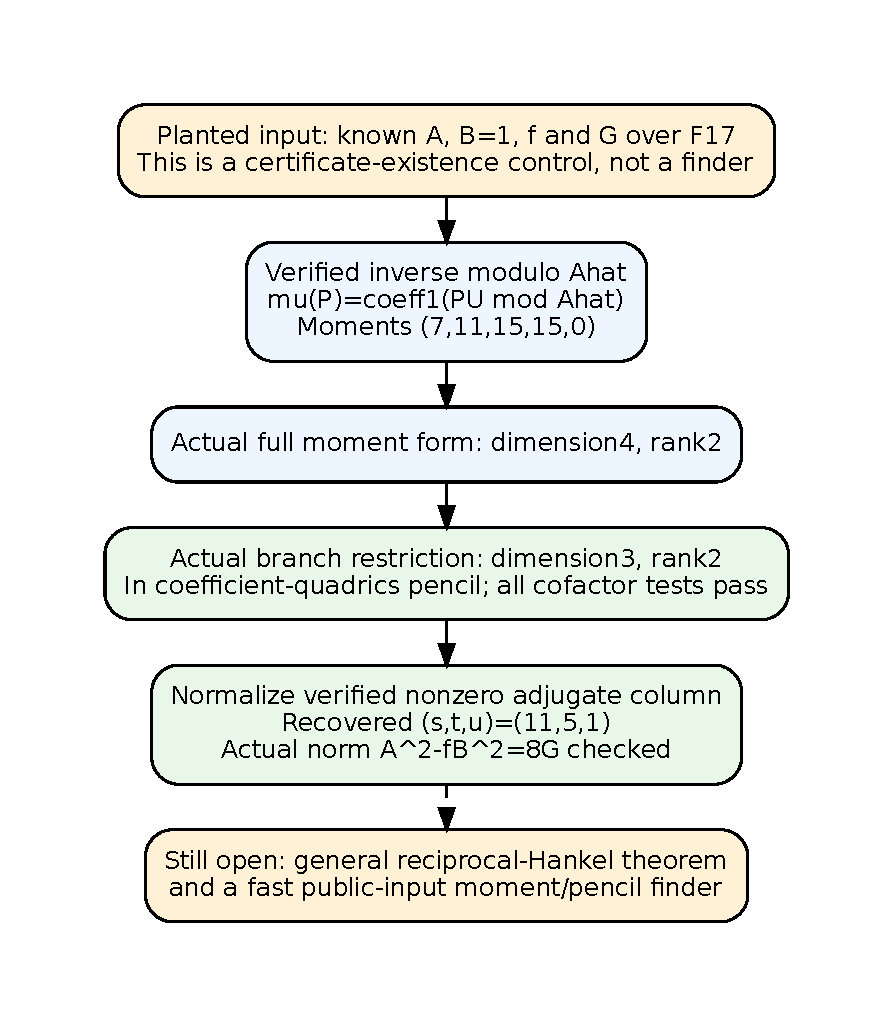
\includegraphics[width=0.94\linewidth,height=0.36\textheight,keepaspectratio]{control.pdf}
\end{center}

\newpage
{\Large Actual coefficient map, rank certificate and evidence}

The full four-dimensional moment form has rank2. Restrict by the actual
branch $A(0)-6B(0)=0$, writing $A=tX^2+sX+6u$, $B=u$. Lean checks the
coefficient equations
\[
 2ts-u^2-3t^2,\quad s^2+12tu-12t^2,\quad12su-2u^2-12t^2
\]
and their complete polynomial expansion. Their matrix pencil at parameters
$(15,15,11)$ equals the actual restricted moment matrix
\[
 S=\begin{pmatrix}15&15&15\\15&0&5\\15&5&14\end{pmatrix},\qquad
 \operatorname{adj}S=\begin{pmatrix}9&1&7\\1&2&14\\7&14&13\end{pmatrix}.
\]
Its rank is2, so its corank is1. Every required cofactor pairing vanishes;
the preceding generic recovery theorem is instantiated with all conditions
proved. The normalized third adjugate column is $(11,5,1)$ and the actual
recovered norm equals $8G$. No numerical-rank assumption is used.

\textbf{Formal map.} Module \path{NormQuotientMoment} contains the general
pairing detectors, the quotient/evaluation identity, actual branch restriction,
pencil membership, full/restricted ranks, coefficient expansion, stationarity
and recovered norm. Exact declaration names and hypotheses are in the README.
Module \path{NormQuotientInteger} separately proves the universal integer lifts
used by the native certificates, rather than attaching a stronger integer
claim to a finite-field proof.

\textbf{Evidence.} Core source \path{3d8417de4}; integer source
\path{cbb5e6372}; Lean4.35.0 with unchanged pinned dependencies. Core build005
passed3149 jobs; expanded build passed3151. Actual tracked-source gate passed90
declarations with zero additional trusted axioms. Separate import-inclusive
fresh receipts are retained per module. Earlier theorem declaration hashes
are unchanged. Failed builds and visibility/normalization errors are retained.

Native records \path{IDC1h91f69b513509f342} and
\path{IDC1he7eb817a6f348de6} each have32 statement-derived and32 extra-stream
points with exact universal proof-source hashes. The native checker does not
execute Lean or establish a search bound. All standing is unsigned producer
evidence; claim bindings and full logs are in the versioned evidence directory.

\textbf{Limits and next test.} This is $a=2$ with constant $B$; it does not
establish nontrivial lower-block reciprocity, general degree/chart cases or a
public-input finder. Next: a generic CRT coefficient-reciprocity lemma and its
Hankel-radical consequence. The $2^{o(n)}$ search bound, $n=\lceil\log_2 r\rceil$,
remains absent. No performance claim, paid job or scaling campaign was run.
Sources: pinned monic-division, quotient-coordinate and matrix declarations;
KB unavailable, no novelty asserted for these classical ingredients.
\end{document}
